
\documentclass[12pt]{article}

%%%%%%%%%%%%%%%%%%%%%%%%%%%%%%%%%%%%%%%%%%%%%%%%%%%%%%%%%%%%%%%%%%%%%%%%%%%%%%%
% PACKAGE INCLUDING
%%%%%%%%%%%%%%%%%%%%%%%%%%%%%%%%%%%%%%%%%%%%%%%%%%%%%%%%%%%%%%%%%%%%%%%%%%%%%%%
\usepackage{amsmath}
\usepackage{graphicx}
\usepackage{hyperref}
\usepackage[utf8]{inputenc}
\usepackage[T5]{fontenc}
\usepackage{fancyhdr}
\usepackage{geometry}

\usepackage{csquotes}
\usepackage{listings}
\usepackage{enumitem}
\usepackage{subfiles}
\usepackage{tcolorbox}
\usepackage{colortbl}
\usepackage{float}
\usepackage{circuitikz}
\usepackage{tikz}
\usepackage{bm}
%%%%%%%%%%%%%%%%%%%%%%%%%%%%%%%%%%%%%%%%%%%%%%%%%%%%%%%%%%%%%%%%%%%%%%%%%%%%%%%
% FORMATTING
%%%%%%%%%%%%%%%%%%%%%%%%%%%%%%%%%%%%%%%%%%%%%%%%%%%%%%%%%%%%%%%%%%%%%%%%%%%%%%%
\geometry{
    a4paper,
    total={170mm,250mm},
    left=20mm,
    top=30mm,
 }
\hypersetup{
    colorlinks=true,
    linkcolor=blue,
    filecolor=magenta,      
    urlcolor=blue,
    citecolor=blue
}

\pagestyle{fancy}
\fancyhf{}
\rhead{19CTT4}
\lhead{Mạch Logic}
\rfoot{Trang \thepage}\setlength{\parindent}{0pt}
\setlength{\parskip}{0.3em}
\setlength{\headheight}{15pt}
\graphicspath{ {./images/} }

\setcounter{secnumdepth}{4}
\setcounter{tocdepth}{4}

\usetikzlibrary{matrix,calc}

%%%%%%%%%%%%%%%%%%%%%%%%%%%%%%%%%%%%%%%%%%%%%%%%%%%%%%%%%%%%%%%%%%%%%%%%%%%%%%%
% DEFINE NEW COMMAND
%%%%%%%%%%%%%%%%%%%%%%%%%%%%%%%%%%%%%%%%%%%%%%%%%%%%%%%%%%%%%%%%%%%%%%%%%%%%%%%
\newcommand{\SubItem}[1]{
    {\setlength\itemindent{15pt} \item[-] #1}
}

%isolated term
%#1 - Optional. Space between node and grouping line. Default=0
%#2 - node
%#3 - filling color
\newcommand{\implicantsol}[3][0]{
    \draw[rounded corners=3pt, fill=#3, opacity=0.3] ($(#2.north west)+(135:#1)$) rectangle ($(#2.south east)+(-45:#1)$);
    }


%internal group
%#1 - Optional. Space between node and grouping line. Default=0
%#2 - top left node
%#3 - bottom right node
%#4 - filling color
\newcommand{\implicant}[4][0]{
    \draw[rounded corners=3pt, fill=#4, opacity=0.3] ($(#2.north west)+(135:#1)$) rectangle ($(#3.south east)+(-45:#1)$);
    }

%group lateral borders
%#1 - Optional. Space between node and grouping line. Default=0
%#2 - top left node
%#3 - bottom right node
%#4 - filling color
\newcommand{\implicantcostats}[4][0]{
    \draw[rounded corners=3pt, fill=#4, opacity=0.3] ($(rf.east |- #2.north)+(90:#1)$)-| ($(#2.east)+(0:#1)$) |- ($(rf.east |- #3.south)+(-90:#1)$);
    \draw[rounded corners=3pt, fill=#4, opacity=0.3] ($(cf.west |- #2.north)+(90:#1)$) -| ($(#3.west)+(180:#1)$) |- ($(cf.west |- #3.south)+(-90:#1)$);
}

%group top-bottom borders
%#1 - Optional. Space between node and grouping line. Default=0
%#2 - top left node
%#3 - bottom right node
%#4 - filling color
\newcommand{\implicantdaltbaix}[4][0]{
    \draw[rounded corners=3pt, fill=#4, opacity=0.3] ($(cf.south -| #2.west)+(180:#1)$) |- ($(#2.south)+(-90:#1)$) -| ($(cf.south -| #3.east)+(0:#1)$);
    \draw[rounded corners=3pt, fill=#4, opacity=0.3] ($(rf.north -| #2.west)+(180:#1)$) |- ($(#3.north)+(90:#1)$) -| ($(rf.north -| #3.east)+(0:#1)$);
}

%group corners
%#1 - Optional. Space between node and grouping line. Default=0
%#2 - filling color
\newcommand{\implicantcantons}[2][0]{
    \draw[rounded corners=3pt, opacity=.3] ($(rf.east |- 0.south)+(-90:#1)$) -| ($(0.east |- cf.south)+(0:#1)$);
    \draw[rounded corners=3pt, opacity=.3] ($(rf.east |- 8.north)+(90:#1)$) -| ($(8.east |- rf.north)+(0:#1)$);
    \draw[rounded corners=3pt, opacity=.3] ($(cf.west |- 2.south)+(-90:#1)$) -| ($(2.west |- cf.south)+(180:#1)$);
    \draw[rounded corners=3pt, opacity=.3] ($(cf.west |- 10.north)+(90:#1)$) -| ($(10.west |- rf.north)+(180:#1)$);
    \fill[rounded corners=3pt, fill=#2, opacity=.3] ($(rf.east |- 0.south)+(-90:#1)$) -|  ($(0.east |- cf.south)+(0:#1)$) [sharp corners] ($(rf.east |- 0.south)+(-90:#1)$) |-  ($(0.east |- cf.south)+(0:#1)$) ;
    \fill[rounded corners=3pt, fill=#2, opacity=.3] ($(rf.east |- 8.north)+(90:#1)$) -| ($(8.east |- rf.north)+(0:#1)$) [sharp corners] ($(rf.east |- 8.north)+(90:#1)$) |- ($(8.east |- rf.north)+(0:#1)$) ;
    \fill[rounded corners=3pt, fill=#2, opacity=.3] ($(cf.west |- 2.south)+(-90:#1)$) -| ($(2.west |- cf.south)+(180:#1)$) [sharp corners]($(cf.west |- 2.south)+(-90:#1)$) |- ($(2.west |- cf.south)+(180:#1)$) ;
    \fill[rounded corners=3pt, fill=#2, opacity=.3] ($(cf.west |- 10.north)+(90:#1)$) -| ($(10.west |- rf.north)+(180:#1)$) [sharp corners] ($(cf.west |- 10.north)+(90:#1)$) |- ($(10.west |- rf.north)+(180:#1)$) ;
}


%Empty Karnaugh map 4x4
\newenvironment{Karnaugh}%
{
\begin{tikzpicture}[baseline=(current bounding box.north),scale=0.8]
\draw (0,0) grid (4,4);
\draw (0,4) -- node [pos=0.7,above right,anchor=south west] {cd} node [pos=0.7,below left,anchor=north east] {ab} ++(135:1);
%
\matrix (mapa) [matrix of nodes,
        column sep={0.8cm,between origins},
        row sep={0.8cm,between origins},
        every node/.style={minimum size=0.3mm},
        anchor=8.center,
        ampersand replacement=\&] at (0.5,0.5)
{
                       \& |(c00)| 00         \& |(c01)| 01         \& |(c11)| 11         \& |(c10)| 10         \& |(cf)| \phantom{00} \\
|(r00)| 00             \& |(0)|  \phantom{0} \& |(1)|  \phantom{0} \& |(3)|  \phantom{0} \& |(2)|  \phantom{0} \&                     \\
|(r01)| 01             \& |(4)|  \phantom{0} \& |(5)|  \phantom{0} \& |(7)|  \phantom{0} \& |(6)|  \phantom{0} \&                     \\
|(r11)| 11             \& |(12)| \phantom{0} \& |(13)| \phantom{0} \& |(15)| \phantom{0} \& |(14)| \phantom{0} \&                     \\
|(r10)| 10             \& |(8)|  \phantom{0} \& |(9)|  \phantom{0} \& |(11)| \phantom{0} \& |(10)| \phantom{0} \&                     \\
|(rf) | \phantom{00}   \&                    \&                    \&                    \&                    \&                     \\
};
}%
{
\end{tikzpicture}
}

%Empty Karnaugh map 2x4
\newenvironment{Karnaughvuit}%
{
\begin{tikzpicture}[baseline=(current bounding box.north),scale=0.8]
\draw (0,0) grid (4,2);
\draw (0,2) -- node [pos=0.7,above right,anchor=south west] {bc} node [pos=0.7,below left,anchor=north east] {a} ++(135:1);
%
\matrix (mapa) [matrix of nodes,
        column sep={0.8cm,between origins},
        row sep={0.8cm,between origins},
        every node/.style={minimum size=0.3mm},
        anchor=4.center,
        ampersand replacement=\&] at (0.5,0.5)
{
                      \& |(c00)| 00         \& |(c01)| 01         \& |(c11)| 11         \& |(c10)| 10         \& |(cf)| \phantom{00} \\
|(r00)| 0             \& |(0)|  \phantom{0} \& |(1)|  \phantom{0} \& |(3)|  \phantom{0} \& |(2)|  \phantom{0} \&                     \\
|(r01)| 1             \& |(4)|  \phantom{0} \& |(5)|  \phantom{0} \& |(7)|  \phantom{0} \& |(6)|  \phantom{0} \&                     \\
|(rf) | \phantom{00}  \&                    \&                    \&                    \&                    \&                     \\
};
}%
{
\end{tikzpicture}
}

%Empty Karnaugh map 2x2
\newenvironment{Karnaughquatre}%
{
\begin{tikzpicture}[baseline=(current bounding box.north),scale=0.8]
\draw (0,0) grid (2,2);
\draw (0,2) -- node [pos=0.7,above right,anchor=south west] {b} node [pos=0.7,below left,anchor=north east] {a} ++(135:1);
%
\matrix (mapa) [matrix of nodes,
        column sep={0.8cm,between origins},
        row sep={0.8cm,between origins},
        every node/.style={minimum size=0.3mm},
        anchor=2.center,
        ampersand replacement=\&] at (0.5,0.5)
{
          \& |(c00)| 0          \& |(c01)| 1  \\
|(r00)| 0 \& |(0)|  \phantom{0} \& |(1)|  \phantom{0} \\
|(r01)| 1 \& |(2)|  \phantom{0} \& |(3)|  \phantom{0} \\
};
}%
{
\end{tikzpicture}
}

%Defines 8 or 16 values (0,1,X)
\newcommand{\contingut}[1]{%
\foreach \x [count=\xi from 0]  in {#1}
     \path (\xi) node {\x};
}

%Places 1 in listed positions
\newcommand{\minterms}[1]{%
    \foreach \x in {#1}
        \path (\x) node {1};
}

%Places 0 in listed positions
\newcommand{\maxterms}[1]{%
    \foreach \x in {#1}
        \path (\x) node {0};
}

%Places X in listed positions
\newcommand{\indeterminats}[1]{%
    \foreach \x in {#1}
        \path (\x) node {X};
}

%%%%%%%%%%%%%%%%%%%%%%%%%%%%%%%%%%%%%%%%%%%%%%%%%%%%%%%%%%%%%%%%%%%%%%%%%%%%%%%
% DOCUMENT
%%%%%%%%%%%%%%%%%%%%%%%%%%%%%%%%%%%%%%%%%%%%%%%%%%%%%%%%%%%%%%%%%%%%%%%%%%%%%%%
\title{PHẦN 4: MẠCH LOGIC}

\author{LỚP 19CTT4}

\date{2021–07–05}


\begin{document}
\begin{sloppypar}

\begin{titlepage}
    
    \newcommand{\HRule}{\rule{\linewidth}{0.5mm}} % Defines a new command for the horizontal lines, change thickness here
    
    \center % Center everything on the page
    \vspace*{\fill}
     
    \textsc{\LARGE Đại học Khoa học Tự nhiên}\\[0.2cm]
    \textsc{\large Đại học Quốc gia TP. HCM }\\[1.5cm] 
    \textsc{\Large KHOA CÔNG NGHỆ THÔNG TIN}\\[0.2cm] 
    \textsc{\large LỚP 19CTT4 }\\[0.5cm]
    \HRule \\[0.4cm]
    { \huge \bfseries Tài liệu ôn thi cuối kỳ môn\break 
    Hệ thống máy tính}\\[0.4cm] % Title of your document
    \HRule \\[1.5cm]
    \LARGE \textbf {PHẦN 4: MẠCH LOGIC \\}
    
    \begin{minipage}{1\textwidth}
    \begin{center}
        \LARGE Ngày 05/07/2021
    \end{center}
    \end{minipage}\\[2cm]
    \vspace*{\fill} % Fill the rest of the page with whitespace
    \end{titlepage}


    % MỤC LỤC
    \renewcommand*\contentsname{\begin{center} \LARGE Mục lục \end{center}}
    \tableofcontents
    \pagebreak
\section{Khái niệm mạch số}

Là thiết bị điện tử hoạt động với \textcolor{red}{2 mức điện áp:}

\begin{itemize}

    \item \textcolor{red}{Cao:} thể hiện bằng giá trị luận lý (quy ước) là \textcolor{red}{1}.
    \item \textcolor{red}{Thấp:} thể hiện bằng giá trị luận lý (quy ước) là \textcolor{red}{0}. 
\end{itemize}


Được xây dựng từ những thành phần cơ bản là \textcolor{red}{cổng luận lý (logic gate)}
\begin{itemize}
    \item Cổng luận lý là thiết bị điện tử gồm 1/ nhiều tín hiệu đầu vào (input) - 1 tín hiệu đầu ra output.
    \item \textcolor{red}{\begin{math}output = F (input\_1, input\_2, ..., input\_n)\end{math}.}
    \item Tùy thuộc vào cách xử lý của hàm F sẽ tạo ra nhiều loại cổng luận lý.
\end{itemize}

Hiện nay linh kiện cơ bản tạo ra mạch số là \textcolor{red}{transistor}.

\subsection{Cổng luận lý(Logic gate)}



\begin{table}[H]
    \centering
    % \begin{tabular}{|l|l|l|}
    \resizebox{\textwidth}{!}{\begin{tabular}{|l|c|l|}
    \hline
    \multicolumn{1}{|c|}{{\color[HTML]{9A0000} \textbf{Tên cổng}}} & \multicolumn{1}{c|}{{\color[HTML]{9A0000} \textbf{Hình vẽ đại diện}}}                       & \multicolumn{1}{c|}{{\color[HTML]{9A0000} \textbf{Hàm đại số Bun}}}                  \\ \hline
    \rowcolor[HTML]{F7E7B7}
    {\color[HTML]{963400} AND}                                     & \begin{circuitikz} \draw (4,4) node[and port, scale = 0.5] {}; \end{circuitikz}    & \(x.y\) hay \(xy\)                                                                            \\ \hline
    {\color[HTML]{963400} OR}                                      & \begin{circuitikz} \draw (4,4) node[or port, scale = 0.5] {}; \end{circuitikz}     & \(x + y\)                                                                                     \\ \hline
    \rowcolor[HTML]{F7E7B7}
    {\color[HTML]{963400} XOR}                                     & \begin{circuitikz} \draw (0,1) node[xor port, scale = 0.5] {}; \end{circuitikz}    & \(x \oplus y\)                                                                                \\ \hline
    {\color[HTML]{963400} NOT}                                     & \begin{circuitikz} \draw (0,1) node[not port, scale = 0.5] {}; \end{circuitikz}    & \(x'\) hay \(\overline{x}\)                                                                   \\ \hline
    \rowcolor[HTML]{F7E7B7}
    {\color[HTML]{963400} NAND}                                    & \begin{circuitikz} \draw (0,1) node[nand port, scale = 0.5] {}; \end{circuitikz}   & \((x.y)'\) hay \(\overline{xy}\)                                                              \\ \hline
    {\color[HTML]{963400} NOR}                                     & \begin{circuitikz} \draw (0,1) node[nor port, scale = 0.5] {}; \end{circuitikz}    & \((x+y)'\) hay \(\overline{x+y}\)                                                             \\ \hline
    \rowcolor[HTML]{F7E7B7}
    {\color[HTML]{963400} NXOR}                                    & \begin{circuitikz} \draw (0,1) node[nor port, scale = 0.5] {}; \end{circuitikz}    & \((x \oplus y)'\) hay \(\overline{x \oplus y}\)                                                                    \\ \hline
    \end{tabular}}
    \end{table}


\subsection{Bảng chân trị}


\begin{itemize}
    \item \textbf{\textcolor{red}{AND}}
    
    \begin{circuitikz} \draw
        (0,1) node[and port] (myand1) {}
            (myand1.in 1) node [anchor=east] {A}
            (myand1.in 2) node [anchor=east] {B}
            (myand1.out)  node [anchor=west] {out};

        \end{circuitikz}
    \begin{table}[H]
        \centering
        \begin{tabular}{|c|c|
        >{\columncolor[HTML]{F8FF00}}l |}
        \hline
        \cellcolor[HTML]{34CDF9}A & \cellcolor[HTML]{34CDF9}B & out                      \\ \hline
        0                         & 0                         & 0                        \\ \hline
        0                         & 1                         & 0                        \\ \hline
        1                         & 0                         & 0                        \\ \hline
        {\color[HTML]{FE0000} 1}  & {\color[HTML]{FE0000} 1}  & {\color[HTML]{FE0000} 1} \\ \hline
        \end{tabular}
        \end{table}
    \item \textbf{\textcolor{red}{OR}}
    
    \begin{circuitikz} \draw
        (0,1) node[or port] (myor1) {}
            (myor1.in 1) node [anchor=east] {A}
            (myor1.in 2) node [anchor=east] {B}
            (myor1.out)  node [anchor=west] {out};

        \end{circuitikz}

    \begin{table}[H]
        \centering
        \begin{tabular}{|c|c|
        >{\columncolor[HTML]{F8FF00}}l |}
        \hline
        \cellcolor[HTML]{34CDF9}A & \cellcolor[HTML]{34CDF9}B & out                      \\ \hline
        {\color[HTML]{FE0000} 0}  & {\color[HTML]{FE0000} 0}  & {\color[HTML]{FE0000} 0} \\ \hline
        0                         & 1                         & 1                        \\ \hline
        1                         & 0                         & 1                        \\ \hline
        {\color[HTML]{333333} 1}  & {\color[HTML]{333333} 1}  & {\color[HTML]{333333} 1} \\ \hline
        \end{tabular}
        \end{table}
    \item \textbf{\textcolor{red}{NOT}}
    
    \begin{circuitikz} \draw
        (0,1) node[not port] (mynot1) {}
            (mynot1.in 1) node [anchor=east] {A}
            (mynot1.out)  node [anchor=west] {out};

        \end{circuitikz}
    \begin{table}[H]
        \centering
        \begin{tabular}{|c|
        >{\columncolor[HTML]{F8FF00}}l |}
        \hline
        \multicolumn{1}{|c|}{\cellcolor[HTML]{34CDF9}A} & \multicolumn{1}{c|}{\cellcolor[HTML]{F8FF00}out} \\ \hline
        {\color[HTML]{FE0000} 0}                        & {\color[HTML]{329A9D} 1}                         \\ \hline
        {\color[HTML]{329A9D} 1}                        & 0                                                \\ \hline
        \end{tabular}
        \end{table}

    \item \textbf{\textcolor{red}{NAND}}
    
    \begin{circuitikz} \draw
        (0,1) node[nand port] (mynand1) {}
            (mynand1.in 1) node [anchor=east] {A}
            (mynand1.in 2) node [anchor=east] {B}
            (mynand1.out)  node [anchor=west] {out};

        \end{circuitikz}
    \begin{table}[H]
        \centering
        \begin{tabular}{|l|l|
        >{\columncolor[HTML]{F8FF00}}l |}
        \hline
        \cellcolor[HTML]{34CDF9}A & \cellcolor[HTML]{34CDF9}B & out                      \\ \hline
        0                         & 0                         & 1                        \\ \hline
        0                         & 1                         & 1                        \\ \hline
        1                         & 0                         & 1                        \\ \hline
        {\color[HTML]{FE0000} 1}  & {\color[HTML]{FE0000} 1}  & {\color[HTML]{FE0000} 0} \\ \hline
        \end{tabular}
        \end{table}

    \item \textbf{\textcolor{red}{NOR}}
    
    \begin{circuitikz} \draw
        (0,1) node[nor port] (mynor1) {}
            (mynor1.in 1) node [anchor=east] {A}
            (mynor1.in 2) node [anchor=east] {B}
            (mynor1.out)  node [anchor=west] {out};
    
        \end{circuitikz}
    \begin{table}[H]
        \centering
        \begin{tabular}{|l|l|
        >{\columncolor[HTML]{F8FF00}}l |}
        \hline
        \cellcolor[HTML]{34CDF9}A & \cellcolor[HTML]{34CDF9}B & out                      \\ \hline
        {\color[HTML]{FE0000} 0}  & {\color[HTML]{FE0000} 0}  & {\color[HTML]{FE0000} 1} \\ \hline
        0                         & 1                         & 0                        \\ \hline
        1                         & 0                         & 0                        \\ \hline
        {\color[HTML]{333333} 1}  & {\color[HTML]{333333} 1}  & {\color[HTML]{333333} 0} \\ \hline
        \end{tabular}
        \end{table}

    \item \textbf{\textcolor{red}{XOR}}
    
    \begin{circuitikz} \draw
        (0,1) node[xor port] (myxor1) {}
            (myxor1.in 1) node [anchor=east] {A}
            (myxor1.in 2) node [anchor=east] {B}
            (myxor1.out)  node [anchor=west] {out};
    
        \end{circuitikz}
    \begin{table}[H]
        \centering
        \begin{tabular}{|l|l|
        >{\columncolor[HTML]{F8FF00}}l |}
        \hline
        \cellcolor[HTML]{34CDF9}A & \cellcolor[HTML]{34CDF9}B & out                      \\ \hline
        {\color[HTML]{333333} 0}  & {\color[HTML]{333333} 0}  & {\color[HTML]{333333} 0} \\ \hline
        {\color[HTML]{FE0000} 0}  & {\color[HTML]{FE0000} 1}  & {\color[HTML]{FE0000} 1} \\ \hline
        {\color[HTML]{FE0000} 1}  & {\color[HTML]{FE0000} 0}  & {\color[HTML]{FE0000} 1} \\ \hline
        {\color[HTML]{333333} 1}  & {\color[HTML]{333333} 1}  & {\color[HTML]{333333} 0} \\ \hline
        \end{tabular}
        \end{table}
\end{itemize}

\subsection{Lược đồ Venn}

{\centering
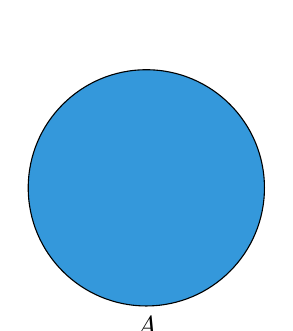
\begin{tikzpicture}
    \definecolor{bluea}{HTML}{3498db}
    % Circle with label at 270 deg.
    \node[draw,
        circle,
        minimum size =3cm,
        fill=bluea,
        label={270:$A$}] (circle1) at (0,-2){};
    \end{tikzpicture}
\begin{tikzpicture}
    \definecolor{bluea}{HTML}{3498db}
    % Circle with label at 270 deg.
    \node[draw,
        circle,
        minimum size =3cm,
        fill=white,
        label={270:$\overline{A}$}] (circle1) at (0,-2){};

    \end{tikzpicture}
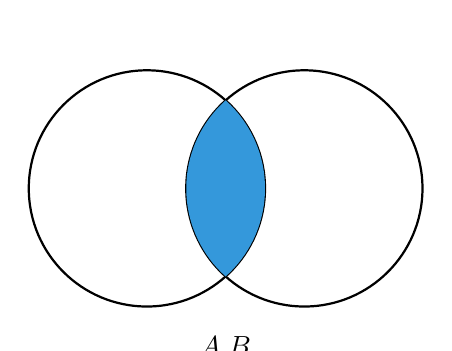
\begin{tikzpicture}[thick]
    \definecolor{bluea}{HTML}{3498db}
    \def\a{1}\def\r{1.5}
    \path (0:\a) coordinate (A) (180:\a) coordinate (B);
    \foreach \x in {A,B} \draw (\x) circle (\r cm);
    \begin{scope}
     \clip (A) circle (\r cm);
     \fill[bluea] (B) circle (\r cm);
    \end{scope}
    \draw (0,-2) node {$A . B$};
    \end{tikzpicture}
}
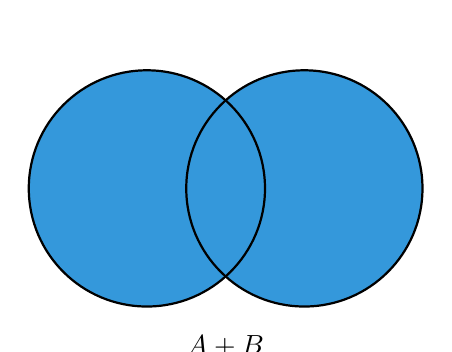
\begin{tikzpicture}[thick]
    \definecolor{bluea}{HTML}{3498db}
    \definecolor{pinkb}{HTML}{8e44ad}
    \def\a{1}\def\r{1.5}
    \path (0:\a) coordinate (A) (180:\a) coordinate (B);
     \fill[bluea] (B) circle (\r cm) (A) circle (\r cm);
     \draw (0,-2) node {$A + B$};
    \foreach \x in {A,B} \draw (\x) circle (\r cm);
    \end{tikzpicture}
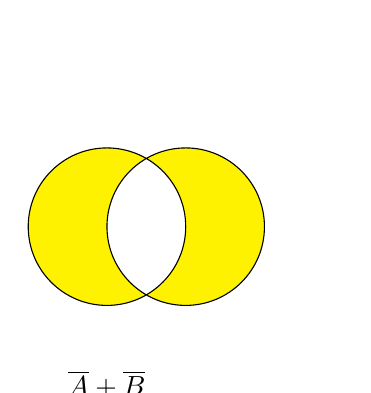
\begin{tikzpicture}[fill=yellow]
    \definecolor{bluea}{HTML}{3498db}

% left hand
    \scope
    \clip (-1,-1) rectangle (3,2)
        (1,0) circle (1);
    \fill (0,0) circle (1);
    \endscope
    % right hand
    \scope
    \clip (-1,-1) rectangle (2,1)
        (0,0) circle (1);
    \fill (1,0) circle (1);
    \endscope
    % outline
    \draw (0,0) circle (1)
        (1,0) circle (1);
    \draw (0,-2) node {$\overline{A} + \overline{B}$};
    \end{tikzpicture}
\subsection{Một số đẳng thức cơ bản}

\begin{table}[H]
    \centering
    %\begin{tabular}{|l|l|}
    \resizebox{\textwidth}{!}{\begin{tabular}{|l|l|}
    \hline
    \rowcolor[HTML]{F7E7B7} 
    $x + 0 = x$                   & $x . 0 = 0$                   \\ \hline
    $x + 1 = 1$                   & $x . 1 = x$                   \\ \hline
    \rowcolor[HTML]{F7E7B7} 
    $x + x = x$                   & $x . x = x$                   \\ \hline
    \rowcolor[HTML]{FFFFFF} 
    $x + x' = 1$                  & $x . \overline{x} = 0$                  \\ \hline
    \rowcolor[HTML]{F7E7B7} 
    $x + y = y + x$               & $xy = yx$                     \\ \hline
    \rowcolor[HTML]{FFFFFF} 
    $x + (y + z) = (x + y) + z$   & $x(yz) = (xy)z$               \\ \hline
    \rowcolor[HTML]{F7E7B7} 
    $x(y + z) = xy + xz$          & $x + yz = (x + y)(x + z)$     \\ \hline
    \rowcolor[HTML]{FFFFFF} 
    $\color{red}\overline{(x + y)} = \overline{x}.\overline{y} (De Morgan)$ & $\color{red}\overline{xy} = \overline{x} + \overline{y} (De Morgan)$ \\ \hline
    \rowcolor[HTML]{F7E7B7} 
    $\overline{\overline{x}} = x$                   &                             \\ \hline
    \end{tabular}}
    \end{table}


\section{Mạch tổ hợp}

\subsection{Khái niệm}
\begin{itemize}
    \item {Gồm \(n\) ngõ vào (input); \(m\) ngõ ra (output)}
        \SubItem {Mỗi ngõ ra là 1 hàm luận lý của các ngõ vào}
    \item {Mạch tổ hợp không mang tính ghi nhớ: Ngõ ra chỉ phụ thuộc vào Ngõ vào hiện tại, không xét những giá trị trong quá khứ}


\end{itemize}

\subsection{Độ trễ mạch}
\begin{itemize}
    \item Độ trễ mạch (\textcolor{red}{Propagation delay/ gate delay}) = Thời gian điểm tín hiệu ra ổn định \(-\) thời điểm tín hiệu vào ổn định.
    \item Mục tiêu thiết kế mạch: làm giảm thời gian độ trễ mạch.
    \subitem \includegraphics[width=9cm]{delay.png}
\end{itemize}

\subsection{Các bước thiết kế}

Thường trải qua 3 bước:
\begin{itemize}
    \item \textcolor{red}{\textbf{Bước 1:} Lập bảng chân trị:}
    \begin{table}[H]
        \centering
        \begin{tabular}{|l|l|
        >{\columncolor[HTML]{F8FF00}}l |}
        \hline
        \cellcolor[HTML]{34CDF9}A & \cellcolor[HTML]{34CDF9}B & F                        \\ \hline
        {\color[HTML]{333333} 0}  & {\color[HTML]{333333} 0}  & {\color[HTML]{333333} 1} \\ \hline
        {\color[HTML]{333333} 0}  & {\color[HTML]{333333} 1}  & {\color[HTML]{333333} 1} \\ \hline
        {\color[HTML]{333333} 1}  & {\color[HTML]{333333} 0}  & {\color[HTML]{333333} 1} \\ \hline
        {\color[HTML]{FE0000} 1}  & {\color[HTML]{FE0000} 1}  & {\color[HTML]{FE0000} 0} \\ \hline
        \end{tabular}
        \end{table}
    \item \textcolor{red}{\textbf{Bước 2:} Viết hàm luận lý} 
    
    \begin{equation*}
        F = \overline{AB}
    \end{equation*}
    
    \item \textcolor{red}{\textbf{Bước 3:} Vẽ sơ đồ mạch và thử nghiệm}
    
    \centering
    \begin{circuitikz} \draw
        (0,1) node[nand port] (mynand1) {}
            (mynand1.in 1) node [anchor=east] {A}
            (mynand1.in 2) node [anchor=east] {B}
            (mynand1.out)  node [anchor=west] {out};
    
        \end{circuitikz}
\end{itemize}

\subsubsection{SOP - Sum of Products}
Giả sử đã có bảng chân trị cho mạch \(n\) đầu vào \textcolor{red}{\(x_{1},...,x_{n}\)} và 1 đầu ra \(f\).
\begin{itemize}
    \item Ta dễ dàng lập công thức (hàm) logic theo thuật toán sau:
    \SubItem {Ứng với mỗi hàng của bảng chân trị có đầu ra = 1, ta tạo thành 1 tích có dạng \(u_{1}.u_{2}...u{n}\)} với:
    \textcolor{red}{
    \[
        f(x)= 
    \begin{cases}
        x_{i},              & \text{nếu } x_{i} = 1 \\
        \overline{x_{i}},   & \text{nếu } x_{i} = 0
    \end{cases}
    \]
    }
    \item \textcolor{red}{Cộng các tích tìm được lại thành tổng -> Công thức của \(f\)}
\end{itemize}
Ví dụ:
\begin{table}[H]
    \begin{tabular}{llll|l}
    \(\textbf{STT}\)            & \multicolumn{1}{r}{\(\boldsymbol{x_{1}}\)}                    & \(\boldsymbol{x_{2}}\) & \(\boldsymbol{x_{3}}\) & \(\boldsymbol{f}\)          \\ \hline
    0                           & 0                      & 0  & 0  & 0                          \\
    \textbf{1}                  & 0                      & 0  & 1  & {\color[HTML]{FE0000} 1}   \(\rightarrow \overline{x_{1}}.\overline{x_{2}}.x_{3}\)                         \\
    \textbf{2}                  & 0                      & 1  & 0  & {\color[HTML]{FE0000} 1}   \(\rightarrow \overline{x_{1}}. x_{2}.\overline{x_{3}}\)                        \\
    3                           & 0                      & 1  & 1  & 0                          \\
    4                           & 1                      & 0  & 0  & 0                          \\
    \textbf{5}                  & 1                      & 0  & 1  & {\color[HTML]{FE0000} 1}   \(\rightarrow x_{1}.\overline{x_{2}}.x_{3}\)                                    \\
    6                           & 1                      & 1  & 0  & 0                          \\
    7                           & 1                      & 1  & 1  & 0                       
    \end{tabular}
    \end{table}
\[\boldsymbol{f = \overline{x_{1}}.\overline{x_{2}}.x_{3} + \overline{x_{1}}. x_{2}.\overline{x_{3}} + x_{1}.\overline{x_{2}}.x_{3} }\]

\subsubsection{POS - Product of Sum}
\begin{itemize}
    \item Trường hợp số hàng có giá trị \textcolor{red}{đầu ra = 1 nhiều hơn = 0}, ta có thể đặt \(g = \overline{f}\).
    \item Viết công thức dạng \textcolor{red}{SOP cho \(g\)}.
    \item Lấy \textcolor{red}{\(f = \overline{g} = \overline{\overline{f}}\)} để có công thức dạng POS (Tích các tổng) của \(f\).
\end{itemize}
Ví dụ: (Thêm sau)
\subsubsection{Đơn giản hóa hàm logic}
\begin{itemize}
    \item Sau khi viết được hàm logic, ta có thể vẽ sơ đồ của mạch tổ hợp từ những cộng luận lý cơ bản.
        \SubItem {Ví dụ: \(f = xy + xz \)} 
    \item Tuy nhiên ta có thể viết lại hàm logic sao cho sơ đồ mạch sử dụng \textcolor{red}{ít cổng hơn}
        \SubItem {Ví dụ: \(f = xy + xz = x(y + z)\)}
    \item Cách đơn giản hóa hàm tổng quát? Một số cách phổ biến:
        \SubItem{Dùng đại số Bun ( Xem lại bảng "Một số đẳng thức cơ bản" để áp dụng)}
        \SubItem{Dùng bản đồ Karnaugh} 
\end{itemize}    

\paragraph{Đại số Bun}
\begin{itemize}
    \item Dùng các phép biển đổi đại số Bun để lược giản hàm logic
    \item Khuyết điểm:
        \SubItem{Không có cách là tổng quát cho mọi bài toán}
        \SubItem{Không chắc kết quả cuối cùng đã tối giản chưa}  
\end{itemize}

\begin{tcolorbox}
    \textbf{Ví dụ:} Đơn giản hóa các hàm sau:
    \(F(x,y,z) = xyz + \overline{x}yz + x\overline{y}z + xy\overline{z}\)
\end{tcolorbox}

\begin{align*}
    F(x,y,z)    & = xyz + \overline{x}yz + x\overline{y}z + xy\overline{z} \\
                & = .....
\end{align*}


\paragraph{Bản đồ Karnaugh}\mbox{}

Mỗi tổ hợp biến trong bảng chân trị gọi là bộ trị(tạm hiểu là 1 dòng)
\begin{itemize}
    \item Biểu diễn hàm có \(n\) biến thì sẽ cho ra tương ứng \(2^{n}\) bộ trị, với vị trí các bộ trị được đánh số từ 0
    \item Thông tin trong bảng chân trị có thể \textcolor{red}{cô đọng} bằng cách:
        \SubItem {Liệt kê vị trí các bộ trị (\textcolor{red}{midterm}) với giá trị đầu ra = \textcolor{red}{1} (\textcolor{red}{SOP})}
        \SubItem {Liệt kê vị trí các bộ trị (\textcolor{red}{maxterm}) với giá trị đầu ra = \textcolor{red}{0} (\textcolor{red}{POS})}
\end{itemize}


\subparagraph{Các dạng bản đồ Karnaugh cơ bản:}
\subparagraph{}

\begin{figure}[H]
\includegraphics[width=4cm]{k_1.png}
\includegraphics[width=5cm]{k_2.png}
\includegraphics[width=6cm]{k_3.png}
\end{figure}

%\begin{Karnaughquatre}
%    \minterms{1,2}
%    \maxterms{0,3}
%    \implicantsol{1}{green}
%    \implicantsol{2}{red}
%\end{Karnaughquatre}

%\begin{Karnaughvuit}
%   \minterms{3,4}
%     \maxterms{0,1,6,7}
%    \indeterminats{2,5}
%    \implicant{3}{2}{green}
%    \implicant{4}{5}{}
%\end{Karnaughvuit}

\begin{tcolorbox}
    \textbf{Ví dụ:} \(F(A,B,C) = \Sigma(1,4,5,6,7) \)
\end{tcolorbox}

%\begin{Karnaughvuit}
%    \minterms{3,4}
%     \maxterms{2,3,4,5,6}
%    \indeterminats{}
%    \implicant{3}{2}{green}
%    \implicant{5}{6}{yellow}
%\end{Karnaughvuit}

\paragraph{Đơn giản hàm theo dạng SOP}

\begin{itemize}
    \item {Hàm logic F biểu diễn bảng chân trị được \textcolor{red}{đưa vào bản đồ bằng các trị 1 tương ứng}.}
    \item Các \textcolor{red}{ô liền kề có giá trị 1 được gom thành nhóm} sao cho mỗi nhóm sau khi gom có \textcolor{red}{tổng số ô là lũy thừa của 2} (2, 4, 8,...).
    \item Các nhóm có thể dùng chung ô có giá trị 1 để gạo thành nhóm lớn hơn. Cố gắng tạo những nhóm lớn nhất có thể.
    \item Nhóm 2/4/8 ô sẽ đơn giản bớt 1/2/3 biến trong số hạng.
    \item \textcolor{red}{Mỗi nhóm biểu diễn 1 số hạng nhân (Product), Cộng(Sum - OR)}, các số hạng này ta sẽ được biểu thức tối giản của hàm logic F.
\end{itemize}


\begin{tcolorbox}
    \textbf{Ví dụ 1:} \(F(A,B,C) = \Sigma(3,4,6,7)\)
\end{tcolorbox}

\includegraphics[width=15cm]{sop_ex1.png}

\begin{equation*}
    \color{red}
    \bm{F(A,B,C) = B.C + A.\overline{C}}
\end{equation*}

\begin{tcolorbox}
    \textbf{Ví dụ 2:} \(F(A,B,C) = \Sigma(0,2,4,5,6)\)
\end{tcolorbox}

\includegraphics[width=15cm]{sop_ex2.png}

\begin{equation*}
    \color{red}
    \bm{F(A,B,C) = \overline{C} + A.\overline{B}}
\end{equation*}

\begin{tcolorbox}
    \textbf{Ví dụ 3:} \(F(A,B,C,D) = \Sigma(0,1,2,6,8,9,10)\)
\end{tcolorbox}

\includegraphics[width=15cm]{sop_ex3.png}

\begin{equation*}
    \color{red}
    \bm{F(A,B,C) = \overline{B}.\overline{D} + \overline{B}.\overline{C} + \overline{A}.C.\overline{D}}
\end{equation*}

\paragraph{Đơn giản hàm theo dạng POS}

\begin{itemize}
    \item Đôi khi biểu diễn dạng tổng các tích (SOP) sẽ khó làm khi \textcolor{red}{số bộ trị có đầu ra = 1 < số bộ trị có đầu ra = 0}
        \SubItem {Dùng phương pháp tích các tổng (POS)}
    \item Hoàn toàn giống phương pháp đơn giản hàm theo dạng SOP, chỉ khác ta \textcolor{red}{nhóm các ô liền kề = 0} thay vì 1
        \SubItem {\textcolor{red}{Tìm được \(\overline{F}\)}}
        \SubItem{\color{red}\(\rightarrow F = \overline{\overline{F}}\)}
\end{itemize}

\begin{tcolorbox}
    \textbf{Ví dụ:} \(F(A,B,C,D) = \Sigma(0,1,2,5,8,9,10)\)
\end{tcolorbox}

\includegraphics[width=15cm]{pos_ex.png}

\begin{equation*}
    \color{red}
    \bm{\overline{F(A,B,C)} = CD + B\overline{D} + AB}
\end{equation*}

{\color{red}
\begin{align*}
    \bm{F} & \bm{= \overline{\overline{F}}} \\
      & \bm{= (\overline{A} + \overline{B}).(\overline{C} + \overline{D}).(\overline{B} + D)}
\end{align*}}


\subsection{Một số bài tập thiết kế mạch}
\begin{tcolorbox}
    \textbf{Ví dụ 1:} Thiết kế mạch cộng 2 bits không nhớ 
\end{tcolorbox}

\begin{itemize}
    \item \textbf{Bước 1:} Lập bảng chân trị
    \begin{table}[H]
        \centering
        \begin{tabular}{|l|l|
        >{\columncolor[HTML]{F8FF00}}l |}
        \hline
        \cellcolor[HTML]{34CDF9}A & \cellcolor[HTML]{34CDF9}B & F                        \\ \hline
        {\color[HTML]{333333} 0}  & {\color[HTML]{333333} 0}  & {\color[HTML]{333333} 0} \\ \hline
        {\color[HTML]{333333} 0}  & {\color[HTML]{333333} 1}  & {\color[HTML]{FE0000} 1} \\ \hline
        {\color[HTML]{333333} 1}  & {\color[HTML]{333333} 0}  & {\color[HTML]{FE0000} 1} \\ \hline
        {\color[HTML]{333333} 1}  & {\color[HTML]{333333} 1}  & {\color[HTML]{333333} 0} \\ \hline
        \end{tabular}
        \end{table}
    \item \textbf{Bước 2:} Lập biểu thức
    
    \begin{align*}
        F & = \overline{A}.B + A.\overline{B} \\
          & = A \oplus B
    \end{align*}

    \item \textbf{Bước 3:} Vẽ mạch

    \centering
    \begin{circuitikz} \draw
    
        (0,1) node[xor port] (myxor1) {}
            (myxor1.in 1) node [anchor=east] {A}
            (myxor1.in 2) node [anchor=east] {B}
            (myxor1.out)  node [anchor=west] {out};
        
        \end{circuitikz}
\end{itemize}

\begin{tcolorbox}
    \textbf{Ví dụ 2:} Thiết kế mạch kiểm tra số nguyên không dấu 3 bits có chia hết cho 3
\end{tcolorbox}

\begin{itemize}
    \item \textbf{Bước 1:} Lập bảng chân trị
    \begin{table}[H]
        \centering
        \begin{tabular}{|c|c|c|c|
        >{\columncolor[HTML]{FCFF2F}}c |}
        \hline
        \cellcolor[HTML]{34CDF9}Hệ 10 & \cellcolor[HTML]{34CDF9}A & \cellcolor[HTML]{34CDF9}B & \cellcolor[HTML]{34CDF9}C & F                        \\ \hline
        0                             & 0                         & 0                         & 0                         & {\color[HTML]{FE0000} 1} \\ \hline
        1                             & 0                         & 0                         & 1                         & 0                        \\ \hline
        2                             & 0                         & 1                         & 0                         & 0                        \\ \hline
        3                             & 0                         & 1                         & 1                         & {\color[HTML]{FE0000} 1} \\ \hline
        4                             & 1                         & 0                         & 0                         & 0                        \\ \hline
        5                             & 1                         & 0                         & 1                         & 0                        \\ \hline
        6                             & 1                         & 1                         & 0                         & {\color[HTML]{FE0000} 1} \\ \hline
        7                             & 1                         & 1                         & 1                         & 0                        \\ \hline
        \end{tabular}
        \end{table}
    \item \textbf{Bước 2:} Lập biểu thức
    \begin{align*}
        F & = \overline{A}.\overline{B}.\overline{C} + \overline{A}.B.C + A.B.\overline{C} \\
          & = \overline{A}.\overline{B}.\overline{C} + B.(\overline{A}.C + A.\overline{C}) \\
          & = \overline{A}.\overline{B}.\overline{C} + B.(A \oplus B)
    \end{align*}

    \item \textbf{Bước 3:} Vẽ mạch



\begin{center}
    \tikzset{every picture/.style={line width=0.75pt}} %set default line width to 0.75pt        

    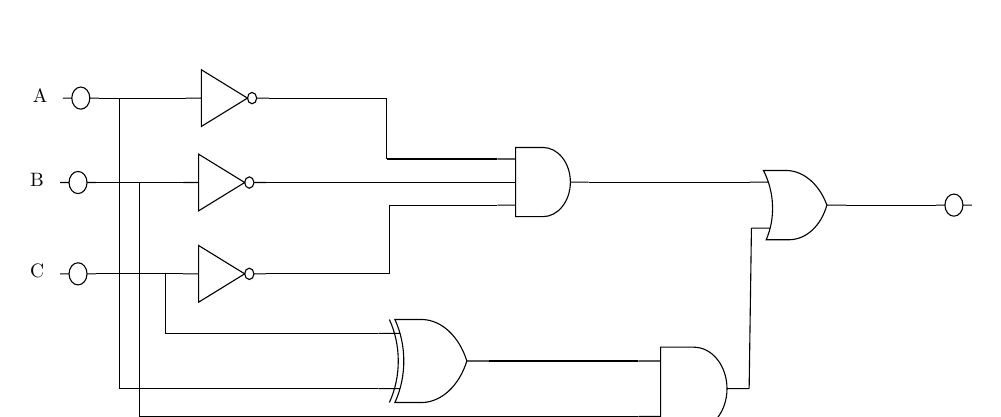
\begin{tikzpicture}[x=0.5pt,y=0.5pt,yscale=-1,xscale=1]
    %uncomment if require: \path (0,310); %set diagram left start at 0, and has height of 310
    
    %Shape: And Gate [id:dp714862170834027] 
    \draw   (365.2,87.67) -- (385,87.67) .. controls (395.93,87.67) and (404.8,98.87) .. (404.8,112.67) .. controls (404.8,126.46) and (395.93,137.67) .. (385,137.67) -- (365.2,137.67) -- (365.2,87.67) -- cycle (352,96) -- (365.2,96) (352,129.33) -- (365.2,129.33) (404.8,112.67) -- (418,112.67) ;
    %Shape: Xor Gate [id:dp8104132100063695] 
    \draw   (278,212) -- (298,212) .. controls (311.95,212.54) and (324.42,224.23) .. (330,242) .. controls (324.42,259.77) and (311.95,271.46) .. (298,272) -- (278,272) .. controls (286.57,253.44) and (286.57,230.56) .. (278,212) -- cycle (266,222) -- (282,222) (266,262) -- (282,262) (330,242) -- (346,242) (274,212) .. controls (282.57,230.56) and (282.57,253.44) .. (274,272) ;
    %Shape: And Gate [id:dp03910276300366866] 
    \draw   (470,232) -- (494,232) .. controls (507.25,232) and (518,245.44) .. (518,262) .. controls (518,278.56) and (507.25,292) .. (494,292) -- (470,292) -- (470,232) -- cycle (454,242) -- (470,242) (454,282) -- (470,282) (518,262) -- (534,262) ;
    %Shape: Not/Inverter Gate [id:dp2824311048801369] 
    \draw   (136.11,92.5) -- (169.44,113) -- (136.11,133.5) -- (136.11,92.5) -- cycle (125,113) -- (136.11,113) (176.11,113) -- (185,113) (169.44,113) .. controls (169.44,110.74) and (170.94,108.9) .. (172.78,108.9) .. controls (174.62,108.9) and (176.11,110.74) .. (176.11,113) .. controls (176.11,115.26) and (174.62,117.1) .. (172.78,117.1) .. controls (170.94,117.1) and (169.44,115.26) .. (169.44,113) -- cycle ;
    %Shape: Output [id:dp5464148080972668] 
    \draw   (42.5,113) .. controls (42.5,108.58) and (45.41,105) .. (49,105) .. controls (52.59,105) and (55.5,108.58) .. (55.5,113) .. controls (55.5,117.42) and (52.59,121) .. (49,121) .. controls (45.41,121) and (42.5,117.42) .. (42.5,113) -- cycle (36,113) -- (42.5,113) (62,113) -- (55.5,113) ;
    %Straight Lines [id:da23347941349353452] 
    \draw    (62,113) -- (125,113) ;
    %Shape: Not/Inverter Gate [id:dp8432013295740557] 
    \draw   (138.11,31.5) -- (171.44,52) -- (138.11,72.5) -- (138.11,31.5) -- cycle (127,52) -- (138.11,52) (178.11,52) -- (187,52) (171.44,52) .. controls (171.44,49.74) and (172.94,47.9) .. (174.78,47.9) .. controls (176.62,47.9) and (178.11,49.74) .. (178.11,52) .. controls (178.11,54.26) and (176.62,56.1) .. (174.78,56.1) .. controls (172.94,56.1) and (171.44,54.26) .. (171.44,52) -- cycle ;
    %Shape: Output [id:dp9659796822269966] 
    \draw   (44.5,52) .. controls (44.5,47.58) and (47.41,44) .. (51,44) .. controls (54.59,44) and (57.5,47.58) .. (57.5,52) .. controls (57.5,56.42) and (54.59,60) .. (51,60) .. controls (47.41,60) and (44.5,56.42) .. (44.5,52) -- cycle (38,52) -- (44.5,52) (64,52) -- (57.5,52) ;
    %Straight Lines [id:da20355845454107624] 
    \draw    (64,52) -- (127,52) ;
    %Shape: Not/Inverter Gate [id:dp7623612408646505] 
    \draw   (136.11,158.5) -- (169.44,179) -- (136.11,199.5) -- (136.11,158.5) -- cycle (125,179) -- (136.11,179) (176.11,179) -- (185,179) (169.44,179) .. controls (169.44,176.74) and (170.94,174.9) .. (172.78,174.9) .. controls (174.62,174.9) and (176.11,176.74) .. (176.11,179) .. controls (176.11,181.26) and (174.62,183.1) .. (172.78,183.1) .. controls (170.94,183.1) and (169.44,181.26) .. (169.44,179) -- cycle ;
    %Shape: Output [id:dp9099392158035657] 
    \draw   (42.5,179) .. controls (42.5,174.58) and (45.41,171) .. (49,171) .. controls (52.59,171) and (55.5,174.58) .. (55.5,179) .. controls (55.5,183.42) and (52.59,187) .. (49,187) .. controls (45.41,187) and (42.5,183.42) .. (42.5,179) -- cycle (36,179) -- (42.5,179) (62,179) -- (55.5,179) ;
    %Straight Lines [id:da9027861118214966] 
    \draw    (62,179) -- (125,179) ;
    %Straight Lines [id:da22161084047882174] 
    \draw    (187,52) -- (272,52) ;
    %Straight Lines [id:da7742552000689296] 
    \draw    (272,96) -- (352,96) ;
    %Straight Lines [id:da7440581637919199] 
    \draw    (272,52) -- (272,96) ;
    %Straight Lines [id:da29746346866587503] 
    \draw    (185,113) -- (365,113) ;
    %Straight Lines [id:da6640846492168198] 
    \draw    (185,179) -- (274,179) ;
    %Straight Lines [id:da2996222203278509] 
    \draw    (274,129.33) -- (352,129.33) ;
    %Straight Lines [id:da04072794070499364] 
    \draw    (274,129.33) -- (274,179) ;
    %Straight Lines [id:da3029481563399097] 
    \draw    (79,52) -- (79,262) ;
    %Straight Lines [id:da313526944530401] 
    \draw    (79,262) -- (266,262) ;
    %Straight Lines [id:da2520687823453367] 
    \draw    (112,222) -- (266,222) ;
    %Straight Lines [id:da2386087614554524] 
    \draw    (112,179) -- (112,222) ;
    %Straight Lines [id:da336692696450523] 
    \draw    (454,242) -- (346,242) ;
    %Straight Lines [id:da3159434314488494] 
    \draw    (93.5,113) -- (93.5,282) ;
    %Straight Lines [id:da12196091116382513] 
    \draw    (93,282) -- (454,282) ;
    %Shape: Or Gate [id:dp43880177207584525] 
    \draw   (544.35,104.33) -- (561.6,104.33) .. controls (573.65,104.78) and (584.8,114.52) .. (590.2,129.33) .. controls (585.98,144.14) and (575.62,153.88) .. (563.6,154.33) -- (546.35,154.33) .. controls (553.13,138.86) and (552.36,119.8) .. (544.35,104.33) -- cycle (534.33,112.67) -- (548.13,112.67) (535.67,146) -- (549.47,146) (590.2,129.33) -- (604,129.33) ;
    %Straight Lines [id:da9993489465543204] 
    \draw    (418,112.67) -- (534.33,112.67) ;
    %Straight Lines [id:da10069054650589204] 
    \draw    (535.67,146) -- (534,262) ;
    %Shape: Output [id:dp5373374461666538] 
    \draw   (675.5,129.33) .. controls (675.5,124.92) and (678.41,121.33) .. (682,121.33) .. controls (685.59,121.33) and (688.5,124.92) .. (688.5,129.33) .. controls (688.5,133.75) and (685.59,137.33) .. (682,137.33) .. controls (678.41,137.33) and (675.5,133.75) .. (675.5,129.33) -- cycle (669,129.33) -- (675.5,129.33) (695,129.33) -- (688.5,129.33) ;
    %Straight Lines [id:da11867269107917533] 
    \draw    (604,129.33) -- (669,129.33) ;
    
    % Text Node
    \draw (13,105) node [anchor=north west][inner sep=0.75pt]  [xscale=0.7,yscale=0.7] [align=left] {B};
    % Text Node
    \draw (15,44) node [anchor=north west][inner sep=0.75pt]  [xscale=0.7,yscale=0.7] [align=left] {A};
    % Text Node
    \draw (13,171) node [anchor=north west][inner sep=0.75pt]  [xscale=0.7,yscale=0.7] [align=left] {C};
    
    
    \end{tikzpicture}
\end{center}
\end{itemize}


\begin{tcolorbox}
    \textbf{Ví dụ 3:} Thiết kế mạch tổ hợp gồm 3 ngõ vào, 1 ngõ ra, sao cho giá trị logic ở ngõ ra là giá trị nào chiếm đa số trong các ngõ vào
\end{tcolorbox}

\begin{itemize}
    \item \textbf{Bước 1:} Lập bảng chân trị
    \begin{table}[H]
        \centering
        \begin{tabular}{|c|c|c|c|
        >{\columncolor[HTML]{FCFF2F}}c |}
        \hline
        \cellcolor[HTML]{34CDF9}Hệ 10 & \cellcolor[HTML]{34CDF9}A & \cellcolor[HTML]{34CDF9}B & \cellcolor[HTML]{34CDF9}C & F                        \\ \hline
        0                             & 0                         & 0                         & 0                         & {\color[HTML]{FE0000} 1} \\ \hline
        1                             & 0                         & 0                         & 1                         & 0                        \\ \hline
        2                             & 0                         & 1                         & 0                         & 0                        \\ \hline
        3                             & 0                         & 1                         & 1                         & {\color[HTML]{FE0000} 1} \\ \hline
        4                             & 1                         & 0                         & 0                         & 0                        \\ \hline
        5                             & 1                         & 0                         & 1                         & 0                        \\ \hline
        6                             & 1                         & 1                         & 0                         & {\color[HTML]{FE0000} 1} \\ \hline
        7                             & 1                         & 1                         & 1                         & 0                        \\ \hline
        \end{tabular}
        \end{table}
        \begin{equation*}
            \color{red}
            \bm{F(x,y,z) = \Sigma(3,5,6,7)}
        \end{equation*}
    \item \textbf{Bước 2:} Lập biểu thức
    
    {\centering \includegraphics[width=15cm]{design_ex3.png}}

    \begin{align*}
        F & = \overline{A}.\overline{B}.\overline{C} + \overline{A}.B.C + A.B.\overline{C} \\
          & = \overline{A}.\overline{B}.\overline{C} + B.(\overline{A}.C + A.\overline{C}) \\
          & = \overline{A}.\overline{B}.\overline{C} + B.(A \oplus B)
    \end{align*}

    \item \textbf{Bước 3:} Vẽ mạch

\begin{center}
    \tikzset{every picture/.style={line width=0.75pt}} %set default line width to 0.75pt        

    \begin{tikzpicture}[x=0.5pt,y=0.5pt,yscale=-1,xscale=1]
    %uncomment if require: \path (0,310); %set diagram left start at 0, and has height of 310
    
    %Shape: Output [id:dp07090963179089083] 
    \draw   (76.88,59.41) .. controls (76.88,55.21) and (79.51,51.82) .. (82.75,51.82) .. controls (85.99,51.82) and (88.63,55.21) .. (88.63,59.41) .. controls (88.63,63.6) and (85.99,67) .. (82.75,67) .. controls (79.51,67) and (76.88,63.6) .. (76.88,59.41) -- cycle (71,59.41) -- (76.88,59.41) (94.5,59.41) -- (88.63,59.41) ;
    %Shape: Output [id:dp3077996138330583] 
    \draw   (73.88,152.41) .. controls (73.88,148.21) and (76.51,144.82) .. (79.75,144.82) .. controls (82.99,144.82) and (85.63,148.21) .. (85.63,152.41) .. controls (85.63,156.6) and (82.99,160) .. (79.75,160) .. controls (76.51,160) and (73.88,156.6) .. (73.88,152.41) -- cycle (68,152.41) -- (73.88,152.41) (91.5,152.41) -- (85.63,152.41) ;
    %Shape: Output [id:dp10121480473965216] 
    \draw   (74.88,259.41) .. controls (74.88,255.21) and (77.51,251.82) .. (80.75,251.82) .. controls (83.99,251.82) and (86.63,255.21) .. (86.63,259.41) .. controls (86.63,263.6) and (83.99,267) .. (80.75,267) .. controls (77.51,267) and (74.88,263.6) .. (74.88,259.41) -- cycle (69,259.41) -- (74.88,259.41) (92.5,259.41) -- (86.63,259.41) ;
    %Shape: Output [id:dp938906996222886] 
    \draw   (584.38,150) .. controls (584.38,145.81) and (587.01,142.41) .. (590.25,142.41) .. controls (593.49,142.41) and (596.13,145.81) .. (596.13,150) .. controls (596.13,154.19) and (593.49,157.59) .. (590.25,157.59) .. controls (587.01,157.59) and (584.38,154.19) .. (584.38,150) -- cycle (578.5,150) -- (584.38,150) (602,150) -- (596.13,150) ;
    %Shape: Or Gate [id:dp0330366347182216] 
    \draw   (175.58,144.85) -- (190.7,144.85) .. controls (201.25,145.25) and (210.68,154.09) .. (214.9,167.53) .. controls (210.68,180.97) and (201.25,189.81) .. (190.7,190.22) -- (175.58,190.22) .. controls (182.06,176.18) and (182.06,158.88) .. (175.58,144.85) -- cycle (166.5,152.41) -- (178.6,152.41) (166.5,182.66) -- (178.6,182.66) (214.9,167.53) -- (227,167.53) ;
    %Shape: Or Gate [id:dp5732518817285119] 
    \draw   (442.08,127.63) -- (457.2,127.63) .. controls (467.75,128.03) and (477.18,136.87) .. (481.4,150.31) .. controls (477.18,163.75) and (467.75,172.59) .. (457.2,173) -- (442.08,173) .. controls (448.56,158.96) and (448.56,141.66) .. (442.08,127.63) -- cycle (433,135.19) -- (445.1,135.19) (433,165.44) -- (445.1,165.44) (481.4,150.31) -- (493.5,150.31) ;
    %Shape: And Gate [id:dp2660962508681879] 
    \draw   (297.6,221.6) -- (315.75,221.6) .. controls (325.77,221.6) and (333.9,231.76) .. (333.9,244.28) .. controls (333.9,256.8) and (325.77,266.97) .. (315.75,266.97) -- (297.6,266.97) -- (297.6,221.6) -- cycle (285.5,229.16) -- (297.6,229.16) (285.5,259.41) -- (297.6,259.41) (333.9,244.28) -- (346,244.28) ;
    %Shape: And Gate [id:dp451149713085919] 
    \draw   (300.6,51.85) -- (318.75,51.85) .. controls (328.77,51.85) and (336.9,62.01) .. (336.9,74.53) .. controls (336.9,87.05) and (328.77,97.22) .. (318.75,97.22) -- (300.6,97.22) -- (300.6,51.85) -- cycle (288.5,59.41) -- (300.6,59.41) (288.5,89.66) -- (300.6,89.66) (336.9,74.53) -- (349,74.53) ;
    %Straight Lines [id:da8112994659907158] 
    \draw    (94.5,59.41) -- (288.5,59.41) ;
    %Straight Lines [id:da47195512550258223] 
    \draw    (91.5,152.41) -- (166.5,152.41) ;
    %Straight Lines [id:da19599155670071444] 
    \draw    (92.5,259.41) -- (285.5,259.41) ;
    %Straight Lines [id:da1036099799156156] 
    \draw    (117.5,152) -- (117.5,229.16) ;
    %Straight Lines [id:da8493424087909229] 
    \draw    (117.5,229.16) -- (285.5,229.16) ;
    %Straight Lines [id:da928850472373969] 
    \draw    (166.5,182.66) -- (166.5,259) ;
    %Straight Lines [id:da3466682598523052] 
    \draw    (227,167.53) -- (227,89.66) ;
    %Straight Lines [id:da32478239181745217] 
    \draw    (288.5,89.66) -- (226.5,89.66) ;
    %Straight Lines [id:da6601193151178855] 
    \draw    (398.5,244.28) -- (346,244.28) ;
    %Straight Lines [id:da37593824158561295] 
    \draw    (349,74.53) -- (398.5,74.53) ;
    %Straight Lines [id:da9039570180032479] 
    \draw    (398.5,165.44) -- (433,165.44) ;
    %Straight Lines [id:da903035916150787] 
    \draw    (398.5,135.19) -- (433,135.19) ;
    %Straight Lines [id:da6637010246104686] 
    \draw    (398.5,74.53) -- (398.5,136) ;
    %Straight Lines [id:da5617997665673444] 
    \draw    (398.5,165.44) -- (398.5,244.28) ;
    %Straight Lines [id:da7581858557033465] 
    \draw    (493.5,150.31) -- (578.5,150) ;
    
    % Text Node
    \draw (40,145) node [anchor=north west][inner sep=0.75pt]  [xscale=0.9,yscale=0.9] [align=left] {Y};
    % Text Node
    \draw (44,252) node [anchor=north west][inner sep=0.75pt]  [xscale=0.9,yscale=0.9] [align=left] {Z};
    % Text Node
    \draw (41,52) node [anchor=north west][inner sep=0.75pt]  [xscale=0.9,yscale=0.9] [align=left] {X};
    
    
    \end{tikzpicture}
\end{center}
\end{itemize}

\subsection{Một số mạch tổ hợp cơ bản}
\subsubsection{Mạch toàn cộng (Full adder)}
\begin{itemize}
    \item Mạch tổ hợp thực hiện phép \textcolor{red}{cộng số học 3 bit}.
    \item Gồm \textcolor{red}{3 ngõ vào} (A,B: bit cần cộng - \(C_{i}\): bit nhớ ) và \textcolor{red}{2 ngõ ra} (kết quả có thể từ 0 đến 3 với giá trị 2 và 3 cần 2 bit biểu diễn -S: ngõ tổng, \(C_{0}\): ngõ nhớ)
\end{itemize}
\subsubsection{Mạch giải mã(Decoder)}
\subsubsection{Mạch mã hóa(Encoder)}
\end{sloppypar}
\end{document}
